\documentclass{article}

\usepackage{hyperref}               % Use hyperlinks

\usepackage[T1]{fontenc}            % Codificação para português 
\usepackage[portuguese]{babel}      % Português

\usepackage{enumitem}               % Corrige indentação dentro de enumerates/itemizes
\setlist{  listparindent=\parindent, parsep=0pt, }

\usepackage{graphicx}               % Coloque figuras
\usepackage{float}                  % Figuras no lugar "esperado"
\graphicspath{{./images/}}          % Localização das imagens

\usepackage[backend=biber, style=authoryear-icomp]{biblatex}
\addbibresource{bibliography/references.bib}
\usepackage{csquotes}               % https://tex.stackexchange.com/a/229653

\usepackage{amsmath}     

\usepackage{enumitem}               % Corrige indentação dentro de enumerates/itemizes
\setlist{  listparindent=\parindent, parsep=0pt, }

\usepackage {tikz}
\usetikzlibrary {positioning}
\definecolor {processblue}{cmyk}{0.96,0,0,0}

\usepackage{multicol}

\author{Luís Felipe Ramos Ferreira }
\title{Trabalho Prático II \\ Algoritmos II \\ Tratamento de problemas difíceis}
\date{November 2022}

\begin{document}

\maketitle

\section{Introdução}

O Trabalho Prático II da disciplina de Algoritmos II teve como objetivo familiarizar os estudantes com o tratamento de problemas difíceis, mais especificamente na implementação dos algoritmos de \texttt{branch-and-bound} e dos algoritmos aproximativos \texttt{twice-around-the-tree} e de \texttt{Christofides}, utilizados na resolução do problema do caixeiro viajante.

A ideia geral do projeto é, além de fazer as implementações, compreender como os resultados variam conforme mudamos os algoritmos, o tamanho das instâncias e os tipos de distância entre os pontos gerados no plano bidimensional.

\section{Implementação}

O trabalho foi feito inteiramente na linguagem de programação Python, versão
3.10.6, no sistema operacional Linux.
Optou-se por serem criados arquivos diferentes para a implementação de cada algoritmo, assim como arquivos diferentes para a ciração de funções auxiliares e do gerador de instâncias. O trabalho não segue nenhuma estrutura de diretórios específica, uma vez que o número de tarefas a serem feitas não exigiam uma organização de arquivos tão detalhada.

Nesa seção, serão discutidos os detalhes da implementação de cada um dos algoritmos, assim como do gerador de instâncias. Algumas referências \footcite{TSP} \footcite{alg} \footcite{youtube} foram utilizadas para compreender melhor os algoritmos, além do conteúdo passado em sala de aula.

\bigskip
\bigskip %Melhorar visualização

\subsection{Gerador de instâncias}

O problema do caixeiro viajante possui diversas variações, mas para o que foi proposto no trabalho iremos lidar com instâncias geométricas do problema. Em outras palavras, cada vértice no grafo será um ponto num espaço euclidiano bidimensional, e as arestas entre cada vértice será a distância entre os pontos representados por eles, podendo essa distância ser a distância euclidiana padrão ou a distância Manhattan.

O gerador de instância utiliza a função \texttt{default-rng} da biblioteca \texttt{numpy} para gerar os pontos no espaço, sem repetição. Com a lista de pontos gerados, são então criadas as matrizes de adjacências, para cada tipo de distância entre os pontos, que representam os grafos da instância. Como as instâncias do caixeiro viajante se baseiam em um grafo completo, devemos preencher a matriz toda para cada caso.

Especificamente para este trabalho, o número de vértices nunca irá exceder 1024, portanto podemos assumir, sem preocupações, que as coordenadas dos pontos varia sempre entre 0 e 5000, tanto para o eixo X como para o eixo Y. 

Para o cálculo das distâncias euclidianas, foi utilizada a função \texttt{dist} da biblioteca \texttt{math}, e para o cálculo da distância Manhattan foi feita uma função auxiliar simples com as próprias funcionalidades da linguagem.

Para exemplificar o que foi discutido, vamos supor que estamos tratando de uma instância com apenas 3 vértices, para fins de simplificade. Os pontos em questão são:

\begin{align*}
    P0 & : (0, 0) \\
    P1 & : (6, 8) \\
    P2 & : (4, 2)
\end{align*}

Considerando essa lista de pontos, temos as seguintes distâncias calculadas se comparados dois a dois:

\begin{multicols}{2}

\textbf{Distância Euclidiana}
\begin{align*}
    P0 - P1 & : 10 \\
    P0 - P2 & : 4.47 \\
    P1 - P2 & : 6.32
\end{align*}

\columnbreak

\textbf{Distância Manhatann}
\begin{align*}
    P0 - P1 & : 14 \\
    P0 - P2 &: 6 \\
    P1 - P2 & : 8
\end{align*}
\end{multicols}

Portanto, para essa instância, teríamos os seguintes grafos considerando cada uma das distâncias:

\bigskip
\bigskip
\bigskip
\bigskip
\bigskip
\bigskip

\begin{center}
    Dist{\^a}ncia Euclidiana
\end{center}

\begin{center}
\begin{tikzpicture}[auto, node distance=3cm, every loop/.style={},
                    thick,main node/.style={circle,draw,font=\sffamily\Large\bfseries}]

  \node[main node] (0) {0};
  \node[main node] (1) [below left of=0] {1};
  \node[main node] (2) [below right of=0] {2};

  \path[every node/.style={font=\sffamily\small}]
    (0) edge [left] node[left] {10.0} (1)
    (1) edge node {4.47} (2)
    (2) edge node [right] {6.32} (0)
;
\end{tikzpicture}
\end{center}

\bigskip
\bigskip % Apenas para melhor visualização do texto
\bigskip

\begin{center}
    Dist{\^a}ncia Manhattan
\end{center}

\begin{center}
\begin{tikzpicture}[auto, node distance=3cm, every loop/.style={},
                    thick,main node/.style={circle,draw,font=\sffamily\Large\bfseries}]

  \node[main node] (0) {0};
  \node[main node] (1) [below left of=0] {1};
  \node[main node] (2) [below right of=0] {2};

  \path[every node/.style={font=\sffamily\small}]
    (0) edge [left] node[left] {14} (1)
    (1) edge node {6} (2)
    (2) edge node [right] {8} (0)
;
\end{tikzpicture}
\end{center}

\bigskip

\subsection{Algoritmos}

Para este trabalho, foi requisitada a implementação de três algoritmos para lidar com instâncias geométricas do problema do caixeiro viajante, as quais serão discutidas a seguir.

\subsubsection{Branch and bound}

O algoritmo de branch and bound para o caixeiro viajante segue a lógica geral de um algoritmo de branch and bound.

Para facilitar a implementação dela, foi criada uma classe \texttt{Node}, a qual representa um nó da árvore de possibilidades. Dentre seus atributos, temos:

\begin{itemize}
\item Estimativa do nó
\item Custo do caminho até o momento
\item Caminho de vértices do grafo até o momento
\item Arestas contabilizadas na estimativa até o momento
\item Vetor de vértices já visitados no caminho
\item Booleano que indica se o vértice 1 já foi visitado
\end{itemize}

Todos os atributos tem por objetivo facilitar o cálculo da estimativa a cada novo nó de possibilidades na árvore, assim como facilitar a podagem de galhos desnecessários. O último atributo, por exemplo, serve para checar se o vértice 1 já foi visitado. Isso é feito para que evitemos qualquer busca que adicione o vértice 0 no caminho sem antes adicionar o vértice 1. Como o caminho hamiltoniano final do caixeiro pode ser encontrado tanto na "ida" como na "volta", podemos assumir que o vértice 1 estará sempre antes do vértice 0, podendo asism evitar computações desnecessárias.

Além dos atributos, essa classe também possui uma sobrecarga do operador \texttt{less than}, de modo a facilitar as comparações na árvore de buscas.

A outra parte principal do algoritmo de branch and bund é o cálculo da estimativa para cada nó da árvore. Inicialmente, calcula-se a estimativa base do grafo como um todo com uma função auxiliar. Então, para cada novo vértice adicionado ao caminho, utiliza-se outra função para atualizar o valor da estimativa com a adição na nova aresta no caminho hamiltoniano.

O algoritmo branch and bound, apesar de evitar buscas desnecessárias, ainda possui uma complexidade exponencial, e portanto possui um custo muito grande para ser executado. Como será detalhado mais a frente, não foi viável testar o algoritmo para instâncias de tamanho 2$^5$ ou maiores.

\subsubsection{Twice around the tree}

O algoritmo \texttt{twice around the tree}, diferentemente do \texttt{branch-and-bound}, é um algoritmo aproximativo para o problema do caixeiro viajante. Mais especificamente, se trata de um algoritmo 2-aproximativo, ou seja, a solução que ele retorna é sempre no máximo duas vezes o custo da solução ótima.

A ideia geral do algoritmo é bem simples, e faz uso da árvore geradora mínima do grafo original e posteriormente de uma busca pré-ordem nessa árvore, a partir de um vértice raiz (no caso deste trabalho, sempre o vértice 0). Para sua implementação, foi utilizada a biblioteca para manipulação de grafos \texttt{networkX}. As funções utilizadas foram a de processamento da árvore geradora mínima do grafo e a de caminhamento pré-ordem.

O gargalo desse algoritmo está no cálculo da árvore geradora mínima, portanto sua execução é bem rápida e bem mais eficiente que o algoritmo de \texttt{branch-and-bound}.

\subsubsection{Christofides}

Assim como o \texttt{twice-around-the-tree}, o algoritmo de \texttt{Christofides} é um algoritmo aproximativo, mas, nesse caso, ele é 1.5-aproximativo. Em outras palavras, a solução que ele retorna é sempre no máximo 1.5 vezes o custo da solução ótima.

A ideia geral do algoritmo é identica à do algoritmo \texttt{twice-around-the-tree}, mas com uma adição que o torna mais preciso. É calculado um matching perfeito de peso mínimo no grafo original entre os vértices de grau ímpar na árvore geradora mínima. A ideia é encontrar o caminho euleriano do multigrafo formado pelas arestas da árvore geradora mínima e do macthing perfeito, e tirar os vértices repetidos.

Mais uma vez, foi utilizada a biblioteca para manipulação de grafos \texttt{networkX}, que possuía todas as funções necessárias já implementadas. Foram utilizadas as mesmas funções do algoritmo \texttt{twice-around-the-tree}, com a adição da função de cálculo do matching perfeito e, agora, ao inves de calcular um caminhamento pré-ordem, é calculado o circuito euleriano do multigrafo euleriano gerado.

O algoritmo possui um gargalo no cálculo do matching perfeito de peso mínimo, o que o torna mais lento que o \texttt{twice-around-the-tree}, mas ainda assim mais rápido que o \texttt{branch-and-bound}.

\section{Experimentos e resultados}

Para analisar as implementações dos algoritmos propostos, foram realizadas diversas baterias de testes, variando entre tamanhos de instância, funções de custo e algoritmos. Para facilitar a visualização dos dados coletados, as informações foram salvas em um \texttt{dataframe} da biblioteca \texttt{pandas}.

Mais especificamente, parada cada tripla (algoritmo, instância, métrica) foram feitos 50 testes e esses dados salvos para análise posterior. O algoritmo de \texttt{branch-and-bound}, no entanto, se mostrou um empecilho para o trabalho. O algoritmo retornava uma resposta apenas para instâncias de tamanho 2$^4$, portanto, para tamanhos maiores, a tabela de dados ficou poluída com NA (não-disponível).

Considerando os detalhes comentados acima, as seguintes tabelas foram obtidas a partir das médias de tempo e custo dos dados coletados de cada algoritmo.

\begin{table}[H]
\centering
\caption{branch-and-bound}
\vspace{0.5cm}
\begin{tabular}{cccc}

Instância & Métrica & Tempo de execu{\c c}{\~a}o (s) & Custo do caminho \\

\hline                          
4 & Euclideana & 99.864 & 18334.2231 \\
4 & Manhattan & 193.251340 & 21574.400 \\
5 a 10 & Euclideana & NA & NA \\
5 a 10 & Manhattan & NA & NA \\

\end{tabular}
\end{table}

\begin{table}[H]
\centering
\caption{twice-around-the-tree}
\vspace{0.5cm}
\begin{tabular}{cccc}

Instância & Métrica & Tempo de execu{\c c}{\~a}o (s) & Custo do caminho \\

\hline                          
4 & Euclideana & 0.000680 & 20830.073 \\
4 & Manhattan & 0.000616 & 26367.400 \\
5 & Euclideana & 0.002286 & 30384.788 \\
5 & Manhattan & 0.002242 & 37640.040 \\
6 & Euclideana & 0.008610 & 42185.425 \\
6 & Manhattan & 0.008620 & 53423.280 \\
7 & Euclideana & 0.038626 & 57672.807 \\
7 & Manhattan & 0.038480 & 73016.800 \\
8 & Euclideana & 0.169828 & 81229.203 \\
8 & Manhattan & 0.171364 & 103205.000 \\
9 & Euclideana & 0.782692 & 114446.829 \\
9 & Manhattan & 0.855336 & 145009.080 \\
10 & Euclideana & 3.683414 & 161266.908 \\
10 & Manhattan & 3.636510 & 204166.160 \\

\end{tabular}
\end{table}

\begin{table}[H]
\centering
\caption{christofides}
\vspace{0.5cm}
\begin{tabular}{cccc}

Instância & Métrica & Tempo de execu{\c c}{\~a}o (s) & Custo do caminho \\

\hline                          
4 & Euclideana & 0.001846 & 18694.113 \\
4 & Manhattan & 0.001736 & 23021.200 \\
5 & Euclideana & 0.006618 & 25733.876 \\
5 & Manhattan & 0.006450 & 31930.360 \\
6 & Euclideana & 0.036902 & 35491.685 \\
6 & Manhattan & 0.039486 & 44118.400 \\
7 & Euclideana & 0.194672 & 48825.996 \\
7 & Manhattan & 0.210878 & 61183.960 \\
8 & Euclideana & 1.005492 & 67525.065 \\
8 & Manhattan & 1.072720 & 85043.160 \\
9 & Euclideana & 6.857486 & 94777.210 \\
9 & Manhattan & 6.872704 & 119532.560 \\
10 & Euclideana & 53.089028 & 132766.232 \\
10 & Manhattan & 48.293676 & 167444.800 \\

\end{tabular}
\end{table}

Os dados coletados na tabela são extremamente úteis para analisar os algoritmos propostos. No entanto, uma apresentação mais visual dos dados permite que conclusães mais assertivas sejam feitas a respeito do que foi coletado. Portanto, alguns gráficos foram gerados com a biblioteca \texttt{pandas} e serão analisados a seguir. É importante ressaltar que, devido ao fato do algoritmo de \texttt{branch-and-bound} ser inviável de realizar testes para grandes instâncias, devido a sua natureza exaustiva, os gráficos englobam principalmente os outros dois algoritmos.

O gráfico abaixo representa a variação do custo dos caminhos gerados pelos algoritmos conforme o aumento do tamanho da instãncia, para cada tipo de função de custo. Os gráficos deixam evidente que o custo dos caminhos considerando a distância Manhattan sao maiores que os considerando a distância Euclideana, o que é natural, uma vez que nossas instâncias geométricas seguem a desigualdade triangular.

\begin{figure} [H]
	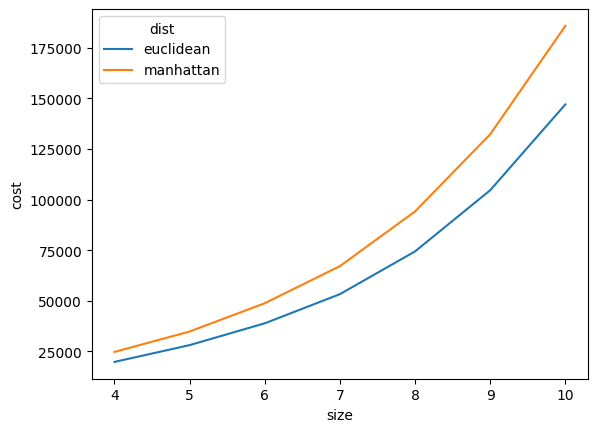
\includegraphics[width=9cm]{images/distdiff.png}
	\centering
\end{figure}

O proximo gráfico mostra como o custo do caminho do caixeiro gerado cresce conforme o tamanho das instâncias crescem, para cada algoritmo. Fica evidente que o algoritmo de \texttt{Christofides} gera caminhos de menor custo que o algoritmo \texttt{twice-around-the-tree}, o que segue o esperado, dado que ele possui um fator de aproximação inferior. Observa-se também, no gráfico subsequente, que embora forneça um caminho de menor custo, o algoritmo de \texttt{Christofides} é bem mais lento, uma vez que o calculo do matching perfeito de peso mínimo possui um custo muito alto de computação. 

\begin{figure} [H]
	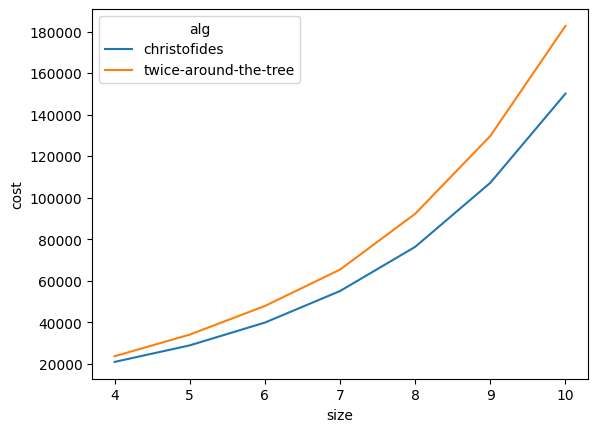
\includegraphics[width=9cm]{images/algcosts.png}
	\centering
\end{figure}

\begin{figure} [H]
	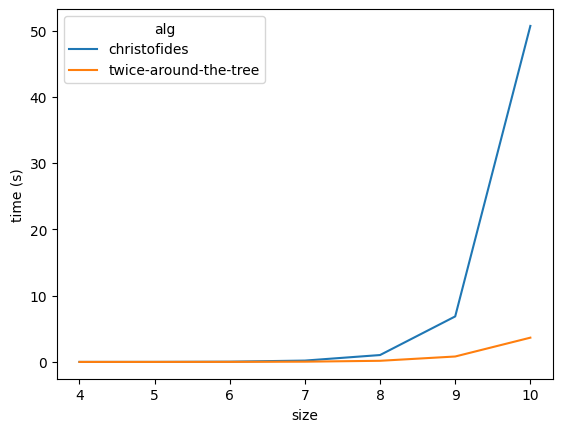
\includegraphics[width=9cm]{images/algtimes.png}
	\centering
\end{figure}

Podemos ver claramente que para instancias de tamanho 2$^{10}$ o tempo de execução do algoritmo de \texttt{Christofides} aumenta de forma explosiva, o que indica que talvez valha a pena utilizar o algoritmo \texttt{twice-around-the-tree} em algumas situações, mesmo que a solução possua um custo de percorrer o caminho maior, já que ele retornaria a resposta em um tempo bem mais factível. No entanto, cada situação possui suas singularidades e cabe ao programador decidir qual o melhor algoritmo para ser utlizado naquele momento.

Por fim, para visualizar a irregularidade do algoritmo de \texttt{branch-and-bound}, a seguinte tabela foi criada, a qual apresenta quanto tempo cada uma das 11 instâncias de tamanho 2$^4$ demorou para ser executada. Podemos ver que esse tempo não segue nenhum padrão, e o algoritmo depende totalmente de uma fator de "sorte", isto é, ser possivel fazer podas na árvore de busca de modo a evitar computações desnecessárias. 

\begin{table}[H]
\centering
\caption{branch-and-bound times}
\vspace{0.5cm}
\begin{tabular}{c}

Tempo de execu{\c c}{\~a}o (s)\\
\hline  
10.7066 \\
2.5554 \\
11.6028 \\
64.5927 \\
130.2230 \\
23.6107 \\
3.0287 \\
47.3529 \\
138.3581 \\
460.3712 \\
683.0441 \\

\end{tabular}
\end{table}

A execução mais rápida para essas especifições demorou 2.5 segundos, enquanto a maislenta demorou 683.04 segundos. São valores muito distantes que demonstram a fragilidade da abordagem de \texttt{branch-and-bound} para o problema.

Em relação a análise de memória na performance dos algoritmos, foi utilizada a biblioteca \texttt{memory-profiler}, que permitia a criação de gráficos de forma rápida que permitiam uma análise assertiva do consumo de memória dos algoritmos.

Para análise e visualização, o custo de memória foi testado para os algoritmos \texttt{twice-around-the-tree} e de \texttt{Christofides} com instâncias de tamanho 2$^{10}$, e estes foram os resultados.

\begin{figure} [H]
	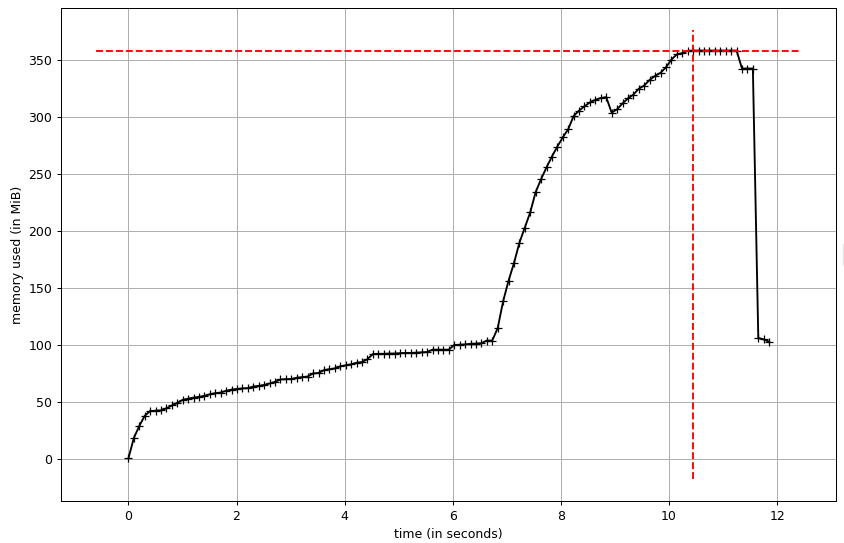
\includegraphics[width=9cm, scale=1.5]{images/tatmem.png}
	\centering
\end{figure}

\begin{figure} [H]
	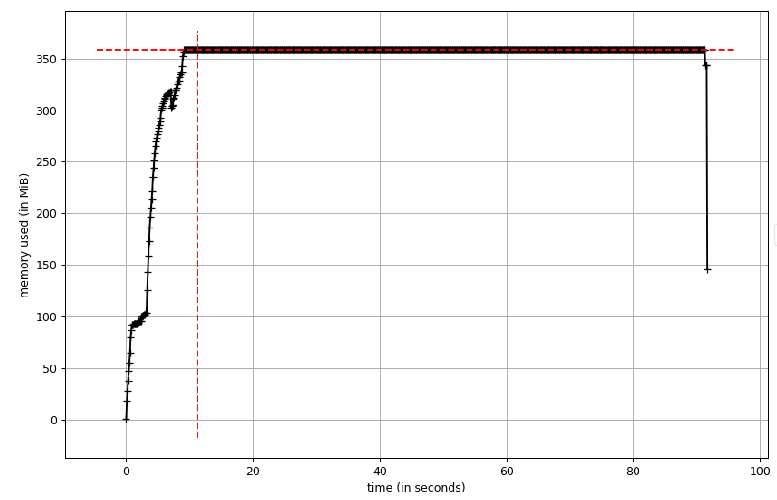
\includegraphics[width=9cm, scale=1.5]{images/crmem.png}
	\centering
\end{figure}

Podemos notar que ambos consumiram uma quantidade similar de memória durante suas execuções, por volta de 350 MiB. Ambos algoritmos possuem implementações semelhantes e não distoam em relação ao consumo de memória.

O algoritmo de \texttt{branch-and-bound}, no entanto, devido a sua natureza exaustiva, consome uma quantidade absurdamente maior de memória. Como podemos ver no gráfico abaixo, para a instância de tamanho 2$^{4}$, ele chega a consumir aproximadamente 580 MiB. Esse também é um dos principais motivos do algoritmo ser inviável para o cálculo do cmainho do caixeiro viajante.

\begin{figure} [H]
	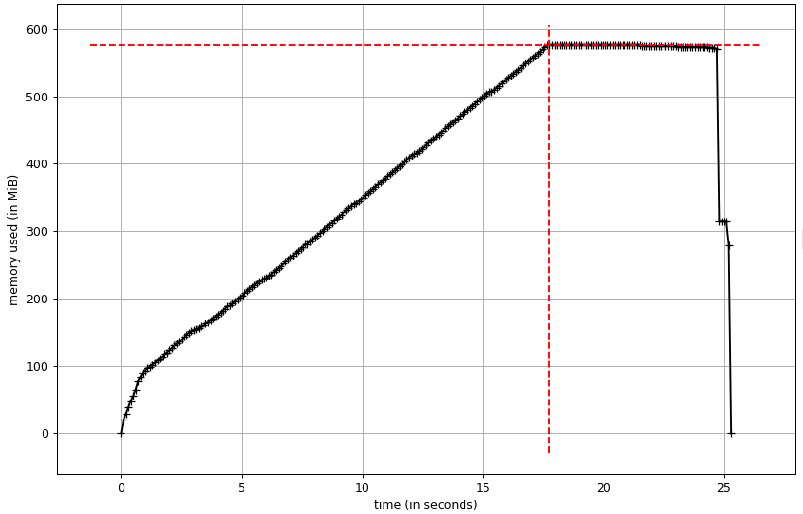
\includegraphics[width=9cm, scale=1.5]{images/bnbmem.png}
	\centering
\end{figure}

\section{Conclusão}

O segundo trabalho prático teve como principal objetivo familiarizar os alunos com o tratamento de problemas difíceis. Em primeiro lugar, é relevante citar como colocar em prática a execução de um algoritmo com complexidade exponencial ajudou a entender o por que desses algoritmos serem ruins. O fato do algoritmo de \texttt{branch-and-bound} ser inviável de testar para instâncias com 2$^{5}$ ou mais vértices mostrou como os algoritmos polinomiais são realmente muito mais factíveis de serem utilizados.

Os outros dois algoritmos que foram implementados, apesar de não retornarem uma solução ótima, possuem um tempo de execução muito menor,  o que para instâncias reais que envolvem mais de 100000 vértices se tornam muito mais plausíveis de serem utilizados.

O segundo ponto importante que se conclui do trabalho é a forma como podemos abordar problema difíceis de maneira inteligente, visando tornar suas resoluções mais viáveis. A ideia de construir um algoritmo aproximativo ainda era meio confusa antes do trabalho, mas enxergar os resultados obtidos mostrou como eles realmente funcionam e são úteis, e por isso grande parte dos pesquisadores trabalham com a otimização desses algoritmos.

Em suma, o trabalho foi crucial para um compreendimento completo da matéria, além de que proporcionou uma visão sobre algoritmos e resolução de problemas que pode ser extendida para diversas outras áreas.

\printbibliography

\end{document}
